\documentclass[letterpaper,twocolumn,fleqn]{article} 

\pagestyle{empty}                % no page numbers is default

\usepackage{amsfonts}
\usepackage{amssymb}
\usepackage[cmex10]{amsmath}
\usepackage{booktabs}
\usepackage{caption}
\usepackage{enumitem}
\usepackage{graphicx}
\usepackage{fancyvrb}
\usepackage{framed}
\usepackage{ifthen}
\usepackage{cite}
\usepackage{tabulary}
\usepackage{url}
\usepackage{xspace}
\usepackage{wrapfig}
\usepackage[pdfborder={0 0 0}]{hyperref}
\usepackage{verbatim}

\usepackage{ist} % Style for IST in package instead of document class.

\usepackage{color}
\definecolor{yellow}{rgb}{1,1,0}
\definecolor{black}{rgb}{0,0,0}
\definecolor{ltcyan}{rgb}{.75,1,1}
\definecolor{red}{rgb}{1,0,0}
\definecolor{gray}{rgb}{.6,.6,.6}
\definecolor{darkred}{rgb}{0.5,0,0}
\definecolor{darkgreen}{rgb}{0,0.5,0}

% Cite commands I use to abstract away the different ways to reference an
% entry in the bibliography (superscripts, numbers, dates, or author
% abbreviations).  \scite is a short cite that is used immediately after
% when the authors are mentioned.  \lcite is a full citation that is used
% anywhere.  Both should be used right next to the text being cited without
% any spacing. \hcite is a citation that I am hiding, perhaps because I am
% nearing the maximum number of citations for a journal.
\newcommand*{\lcite}[1]{~\cite{#1}}
\newcommand*{\scite}[1]{~\cite{#1}}
\newcommand*{\hcite}[1]{}

\newcommand{\etal}{et al.\xspace}

\newcommand*{\keyterm}[1]{\emph{#1}}

\newcommand{\fix}[1]{{\color{red}\textsc{[#1]}}}
%\newcommand{\fix}[1]{}

% Avoid putting figures on their own page.
\renewcommand{\textfraction}{0.05}
\renewcommand{\topfraction}{0.95}
\renewcommand{\bottomfraction}{0.95}

% Make sure this is big enough so that only big figures end up on their own
% page but small enough so that if a figure does have to be on its own
% page, it won't push everything to the bottom because it's not big enough
% to have its own page.
\renewcommand{\floatpagefraction}{.75}


\title{Why We Use Bad Color Maps and What You Can Do About It}

\author{Kenneth Moreland; Sandia National Laboratories; Albuquerque, New
  Mexico, USA}

\date{} % date has an empty field.

% correct for bad hyphenation here
\hyphenation{Para-View}

\begin{document} 

\maketitle 

\thispagestyle{empty} % prevents the first page to be numbered

\begin{abstract}
\noindent
We know the rainbow color map is terrible and emphatically reviled by the
visualization community, yet its use continues to persist. Why do we
continue to use a this perceptual encoding with so many known flaws?
Instead of focusing on why we should not use rainbow colors, this position
statement explores the rational for why we do pick these colors despite
their flaws. Often the decision is influenced by a lack of knowledge, but
even experts that know better sometimes choose poorly. A larger issue is
the expedience that we have inadvertently made the rainbow color map
become. Knowing why the rainbow color map is used will help us move away
from it. Education is good, but clearly not sufficient. We gain traction by
making sensible color alternatives the more convenient alternative. It is
not feasible to force a color map on users. Our goal is to supplant the
rainbow color map as a common standard, and we will find that even those
wedded to it will migrate away.
\end{abstract}


\section{Introduction}

\noindent
A pervasive technique in scientific visualization called pseudocoloring is
to apply colors to an object that vary based on some numerical variable.
Pseudocoloring requires defining a function or map from numerical values to
colors. A color map is typically defined by selecting a continuum of colors
that map linearly to a range of numeric values.
Figure~\ref{fig:ColorMapExample} shows a simple example of a color map
where numeric values between -1 and 0 map to blue colors of varying
brightness and numeric values between 0 and 1 map to red colors.

\begin{figure}[htb]
  \centering
  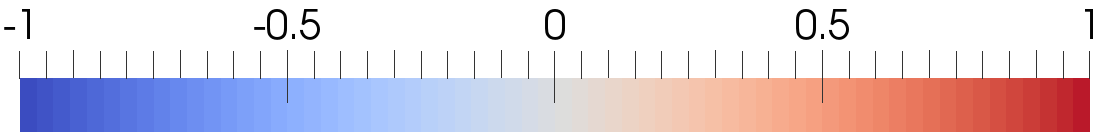
\includegraphics[width=.9\linewidth]{images/ColorMapExample}
  \caption{A simple example of a color map.}
  \label{fig:ColorMapExample}
\end{figure}

The efficacy of a pseudocolor visualization is contingent on the ability of
a human observer to translate the colors back into the numeric values they
represent. The choice of colors used in a pseudocolor map can have a major
impact on this inverse translation. Consequently, much research has focused
on the perception of color and its impact of the visual display of
data\fix{cite stone, brewer, ware, reigens, rogowitz}. As one might expect,
the color choice can have a dramatic impact on a viewer's performance in
interpreting colors as numbers, and many effective color sets have been
designed for this purpose.

With this rich understanding of color perception, one might think that
modern visualizations make effective use of color. Unfortunately, many
visualizations today use color sets that are known to be extremely
problematic. In particular the rainbow color map, so called for its use of
the spectrum of colors in the rainbow, is pervasively used in visualization
despite the copious evidence that it performs poorly\fix{cite Borland,
  Reigens, Franchesca? Others?}.

This paper is a retrospective on why these bad colors are so commonly
chosen for visualization and is a position statement on what we as
practitioners can do to best promote good color use.

\fix{I am considering having a short section on the evils of the rainbow
  color map if there is room. If I do, I might remove a few lines above. If
  I do not, I might add a statement or two above that we are not addressing
  this because it is so commonly presented.}


\section{Why We Use Bad Colors}

\noindent
Reserach shows that subjects tend to overestimate their ability to
interpret rainbow colors\fix{cite}. That is, users think they are
interpreting rainbow colors better than alternatives even though they are
in fact doing worse. This is certainly a contributing factor to the
proliferation of the rainbow color map, but not the entire reason. Why else
would the rainbow color map be so profuse in publications by the
visualization community itself, a community that should know
better\fix{cite Borland}?

One explanation is the sheer simplicity of creating the rainbow color map.
Nearly all color selections in computer graphics interfaces are done with
RGB (red-green-blue) channels. RGB is a natural choice in computer graphics
because the triplet values match the intensity of red, green, and blue
light mixed in most display peripherals. An unintended consiquence of the
RGB color space is that one of the easiest color continua to make is an
interpolation between different combinations of fully active and fully
inactive channels, which are in fact the rainbow colors. Many computer
graphics interfaces also allow colors chosen with HSV
(hue-saturation-value) channels. The HSV color space makes makes rainbow
colors even easier: hold saturation and value at maximum while varying hue.

With the simplicity of creating a rainbow spectrum of colors combined with
the inclination to accept the colors as a good representation, it is no
wonder that the rainbow colors are often the first and likely the default
color mapping introduces as a visualization package gets built. These
initial poor color choices quickly become ingrained in the software as
regression testing and backward compatibility must be maintained. Further
software layers continue to accept this default and software applications
are likely to expose the rainbow color map as its default choice for end
users. Few users will have either the knowledge or the inclination to
change the default colors used, and thus the rainbow color map becomes
featured throughout visualizations.

However, simplicity is not the only reason rainbow colors are so widely
used. If that were the case, simply making a better alternative would
eradicate the use of bad colors. But this, at least anecdotally, is shown
not to be the case. Consider, for example, bug number 7024 for the ParaView
scientific visualization
application.\footnote{\url{http://www.paraview.org/Bug/view.php?id=7024}} A
user raised this bug soon after the default color map in ParaView was
changed from the rainbow color map to the map shown in
Figure~\ref{fig:ColorMapExample}, which is designed to be reasonably
similar to the rainbow color map it supplants but with better perceptual
characteristics\fix{cite my paper, perceptual studies on it}. Despite this
movement to make the better color map easier, this bug report is an
artifact of the user's difficulty as he went through the extra motions to
go back to the rainbow color map.

The overestimation of the efficacy of the rainbow color map might be a
motivator to spend effort to go back to it, but it is unlikely to be a very
strong motivator. In fact, other ancdotal incidents suggest that even users
that are aware of the rainbow's flaws still have an affinity to use it.
\fix{Throw Alan under the bus.}

\fix{Still not sufficent. Counterexamples of bug reports, intentionally
  chosen colors (apple).}

\fix{Of course, interpretation. Ultimately, people like the aesthetics.
  Oooh, shiney. And sciency.}

\fix{Also, communities sometimes get ``stuck'' in color choices. Need to
  compare current visualization with those generated 10 years ago.}

\fix{Should there be subsections that act like an enumeration for tl;dr?}


\section{How We Can Promote Good Color Use}


\section{Practical Considerations}

\fix{Managing the unknown.}

\fix{Contending with asthetics.}


\section{Acknowledgments} 

% To start a new column (but not a new page) and help balance the last-page
% column length use \vfill\pagebreak.

\small
\bibliographystyle{plain}
%% \bibliography{BadColorMaps}

\begin{biography}
\noindent
Dr. Kenneth Moreland is a principal member of technical staff at Sandia
National Laboratories. He received the BS degrees in computer science and
electrical engineering from New Mexico Tech in 1997. He received MS and
Ph.D. degrees in computer science from the University of New Mexico in
2000, and 2004, respectively. Dr. Moreland specializes in large-scale
visualization and plays an active role in several HPC products including
ParaView, VTK, IceT, Dax, and VTK-m.
\end{biography}

\end{document} 
